\section{Simulation Analysis}
\label{sec:simulation}

\hspace{0,5cm} This section covers the audio amplifier circuit simulation using the Ngspice tool.
\par As asked in the lab assignment, a NPN transistor and a PNP transistor were used in gain stage and output stage respectively. The goal was to calculate the impedances ($Z_I$ and $Z_O$), the cut off frequencies (), the bandwidth (the difference between the cut off frequencies) and the total gain.
\par It was also confirmed if the BJTs are on the F.A.R. (forward active region) by comparing $V_{CE}$ and $V_{BE}$ for NPN type and $V_{EC}$ and $V_{EB}$ for PNP type.
\par Later in this report, we will compare this results with the theoretical ones but for now we will just show them.

\par The Table~\ref{tab:ng2} and \ref{tab:ng3} shows the BJTs voltages and their F.A.R. confirmation.

\begin{table}[!ht]
  \centering
  \begin{tabular}{|l|r|}
    \hline    
    {\bf Name} & {\bf Value [A or V]} \\ \hline
    V(CE) & 2.78156\\ \hline
V(BE) & 0.70931\\ \hline
V(CE)>V(BE) & Yes\\ \hline

  \end{tabular}
  \caption{F.A.R. confirmation - BC547A (NPN type)}
  \label{tab:ng2}
\end{table}

\begin{table}[!ht]
  \centering
  \begin{tabular}{|l|r|}
    \hline    
    {\bf Name} & {\bf Value [A or V]} \\ \hline
    V(EC) & 4.49605\\ \hline
V(EB) & 0.817257\\ \hline
V(EC)>V(EB) & Yes\\ \hline

  \end{tabular}
  \caption{F.A.R. confirmation - BC557A (PNP type)}
  \label{tab:ng3}
\end{table}

\par In the next table it is presented the results asked.

\begin{table}[!ht]
  \centering
  \begin{tabular}{|l|r|}
    \hline    
    {\bf Name} & {\bf Value [A or V]} \\ \hline
    V_Gain&37.9181\\ \hline
Bandwidth&1.55393E+06\\ \hline
CO_Freq& 8793.49\\ \hline

  \end{tabular}
  \caption{Ngspice simulation results}
  \label{tab:ng4}
\end{table}

\par The merit obtained by the groups is presentend in the following table.

\begin{table}[!ht]
  \centering
  \begin{tabular}{|l|r|}
    \hline    
    {\bf Name} & {\bf Value [A or V]} \\ \hline
    Cost & 123.208\\ \hline
merit & 54.3849\\ \hline

  \end{tabular}
  \caption{Cost and merit results}
  \label{tab:ngs1}
\end{table}


\begin{figure}[ht!] \centering
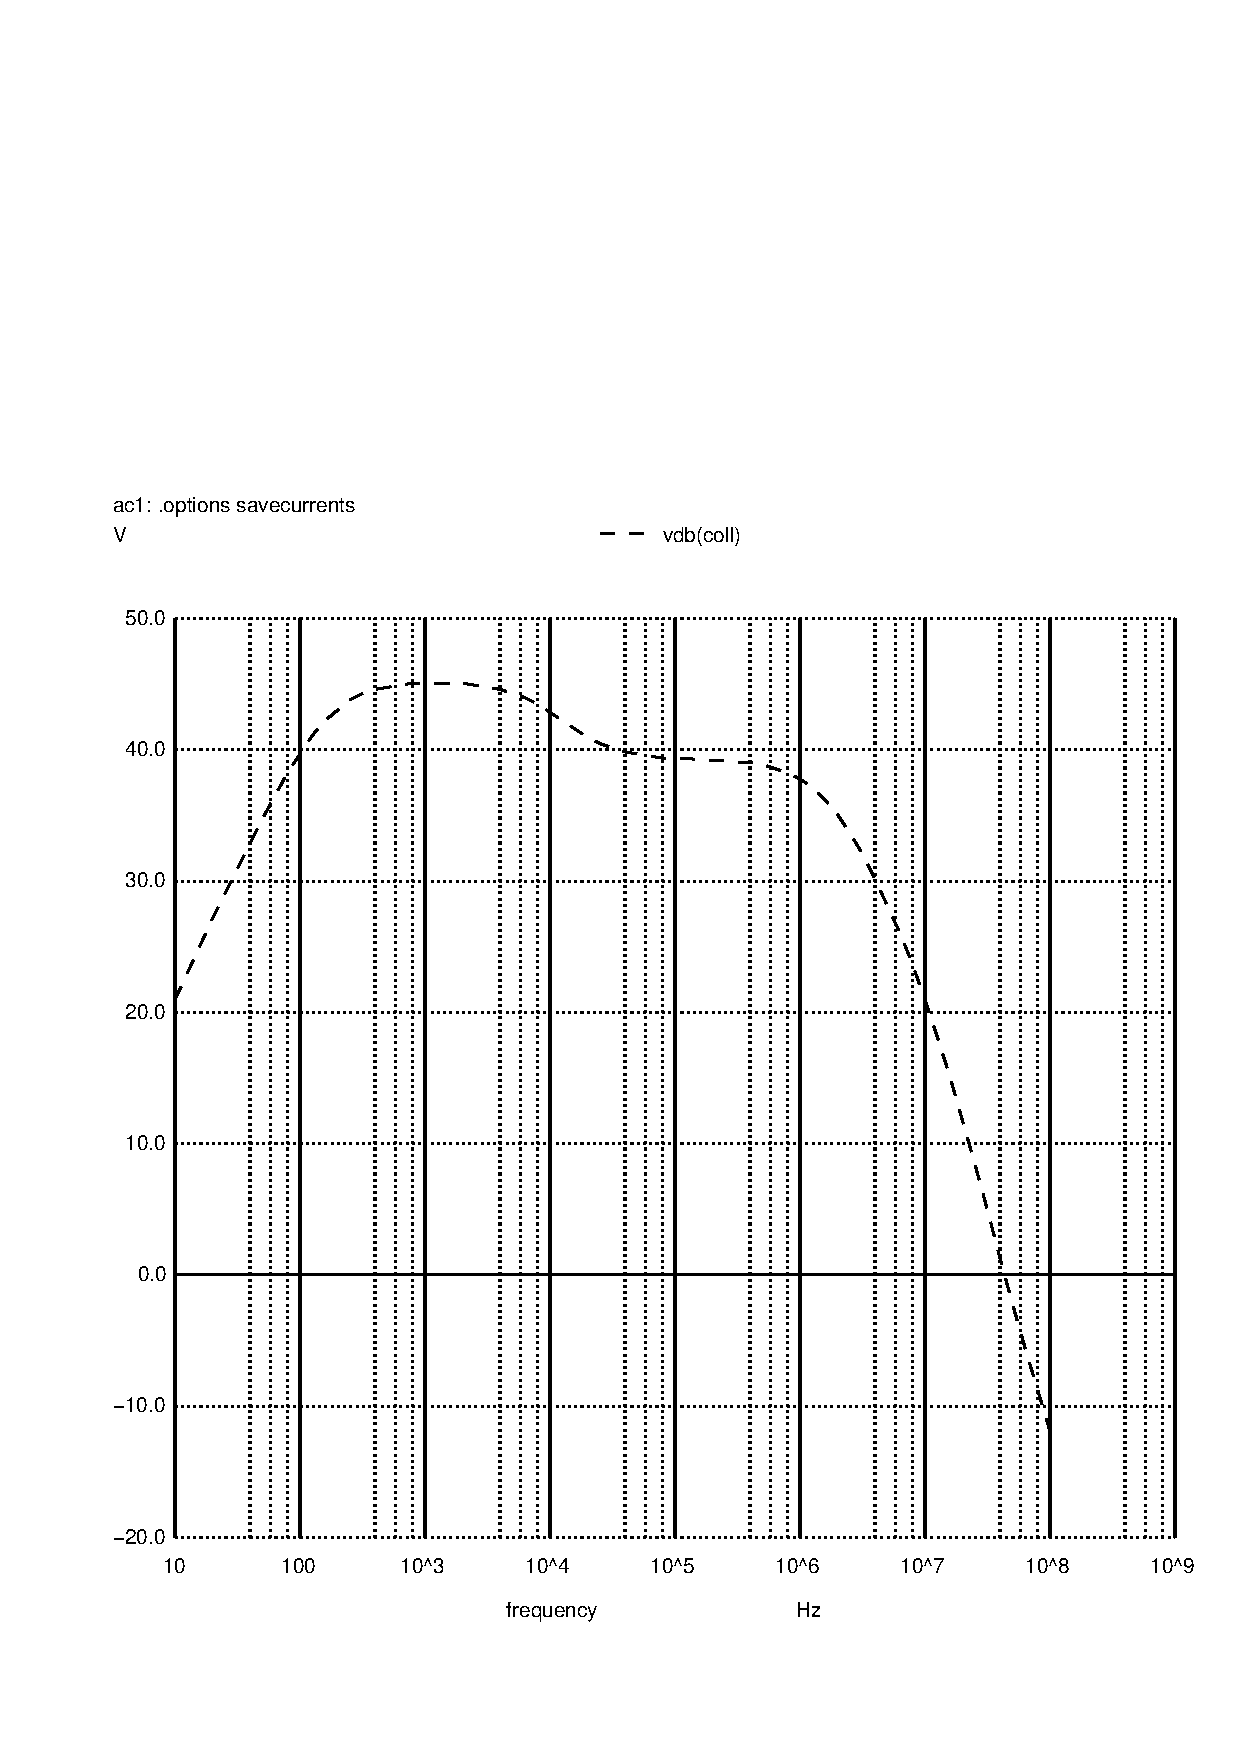
\includegraphics[width=0.5\linewidth]{../sim/vo1f.pdf}
\caption{Output Voltage of the envelope detector v(4)} 
\label{fig:sim1}
\end{figure}

\begin{figure}[ht!] \centering
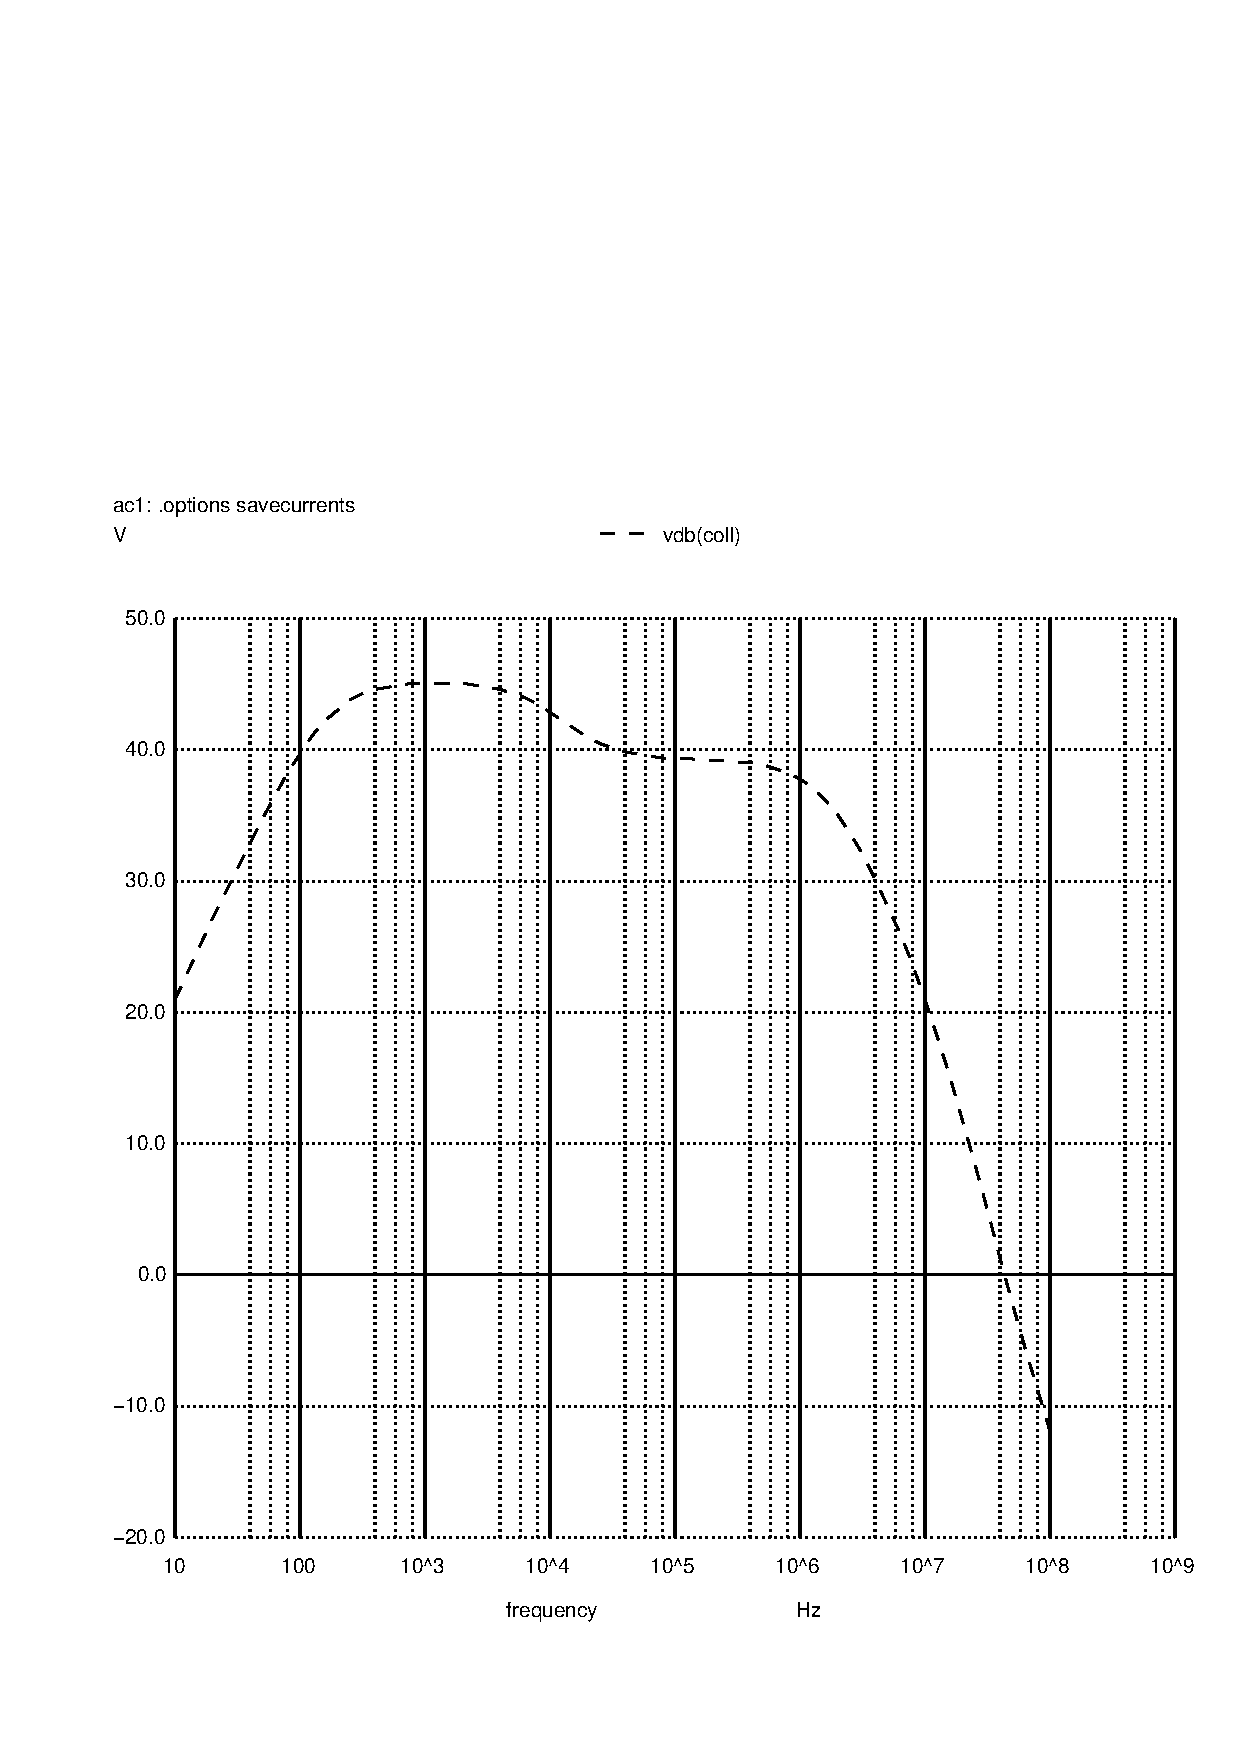
\includegraphics[width=0.5\linewidth]{../sim/vo2f.pdf}
\caption{Input Voltage of the secondary circuit (v(2)-v(3))} 
\label{fig:sim2}
\end{figure}

\begin{table}[!ht]
  \centering
  \begin{tabular}{|l|r|}
    \hline    
    {\bf Name} & {\bf Value [A or V]} \\ \hline
    Zin & -548.062 + 82.7641 j\\ \hline

  \end{tabular}
  \caption{Merit values}
  \label{tab:ng5}
\end{table}


